\begin{scriptsize}
    \begin{center}
        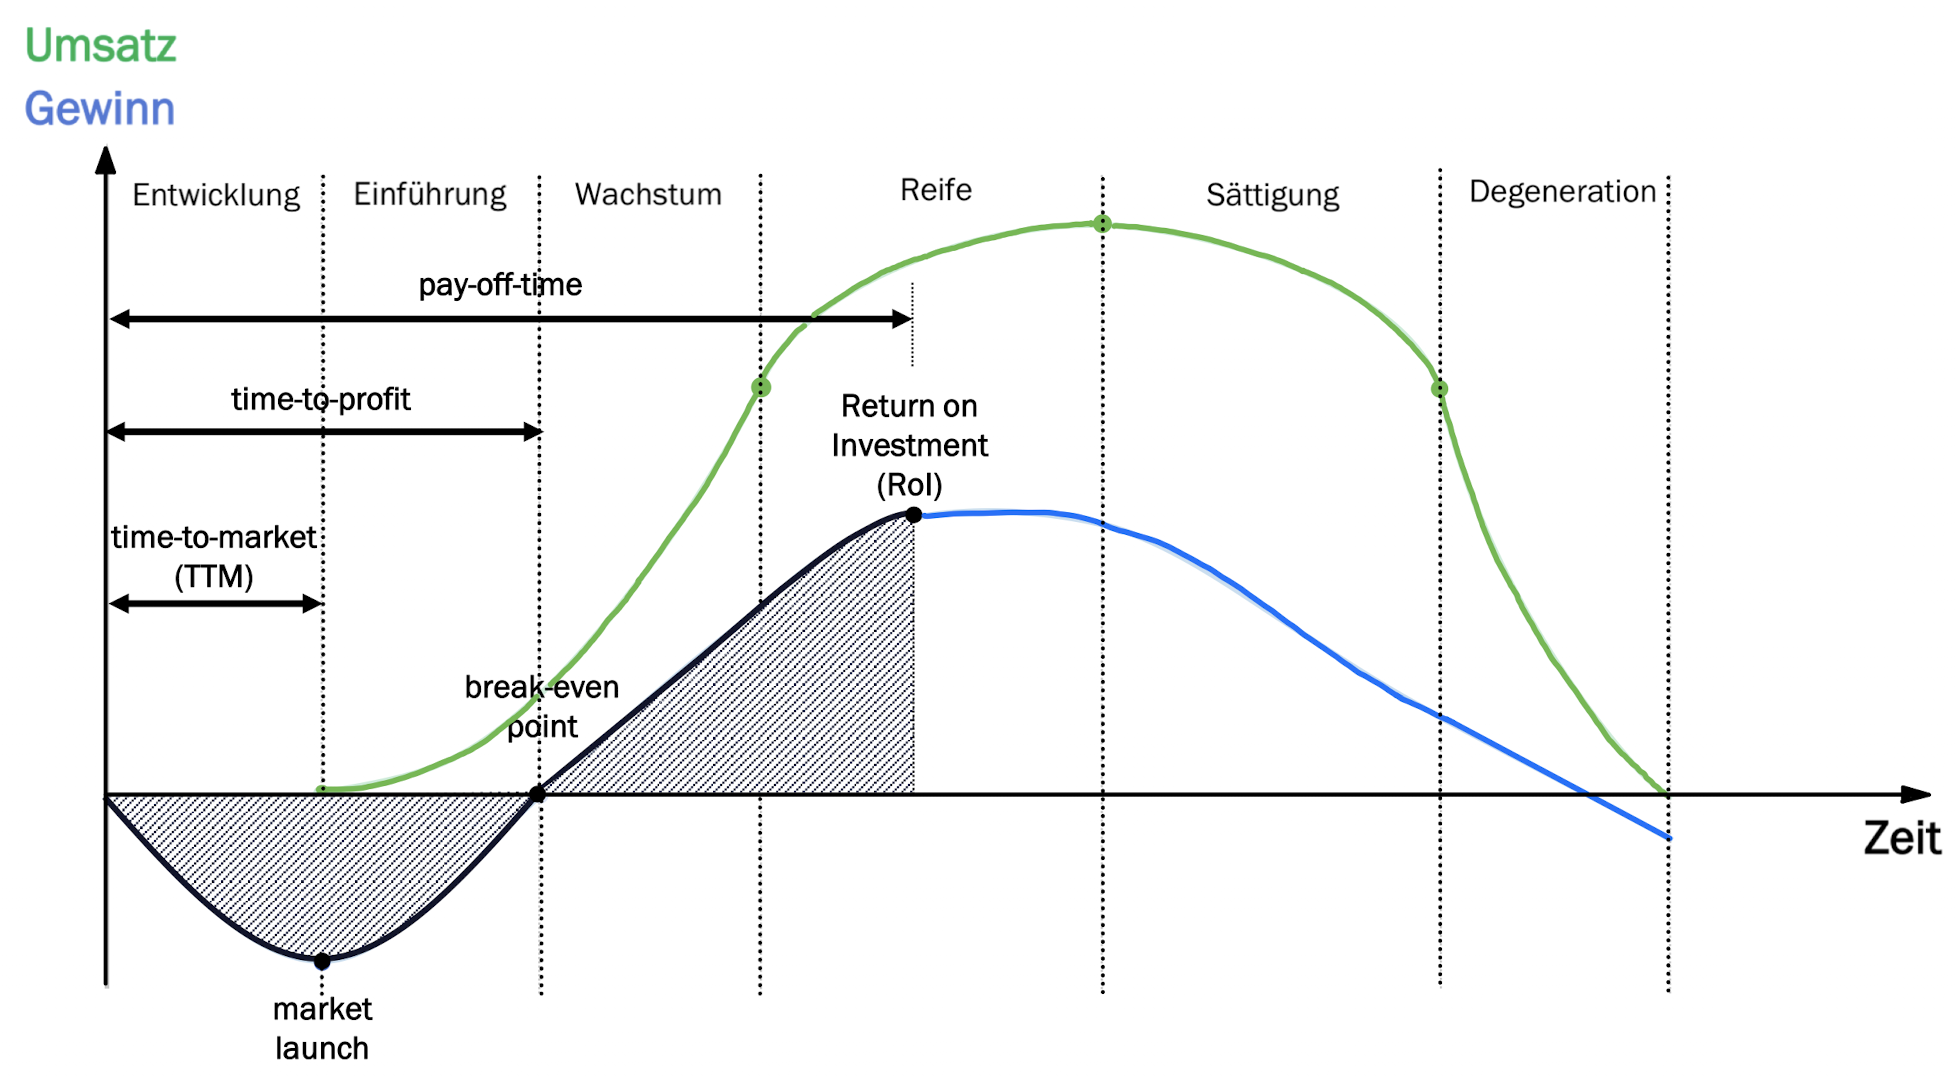
\includegraphics[width = 0.9\linewidth]{MAEIP_Produktlebenszyklus}
    \end{center}
    \begin{itemize}
        \item \textbf{Enwicklung:} Investition in Entwicklung / Fertigung der norwendigen Maschinen und Mitarbeiter / endet mit market-launch
        \item \textbf{Einführung:} geringer Absatz / Produkt etabliert sich durch Werbung, etc. / endet mit break-even Positionierungsgenauigkeit
        \item \textbf{Wachstum:} Verkaufszahlen nehmen zu / Investition in Werbung / Ausbau Produk-\\tion / endet, wenn Wachstumsrate rückläufig
        \item \textbf{Reife:} am ertragreichsten, da hoher Umsatz mit weniger Investitionen / endet, wenn \\Umsatz rückläufig
        \item \textbf{Sättigung:} Umsatz und Gewinn nehmen ab / Produkt muss modifiziert oder durch \\Nachfolgeprodukt ersetzt werden
        \item \textbf{Degeneration:} Umsatz und Gewinn brechen ein / Produkt sollte vom Markt \\genommen werden / Ausnahme: Produkt trägt zu Imagegeinn bei
    \end{itemize}
\end{scriptsize}